\subsection{Performance of the Filter}
The position Kalman filter is tested in a similar way as the attitude one. The simulations have been performed by applying some inputs to the simulation model of the system. The signals coming out of the model are then extracted and some noise is added to them. The noisy signals are used as the input to the position Kalman filter in order to evaluate its performance. The amount of noise added is the same as that present in the real sensors, the variance values can be seen in \autoref{app:IMUvariances}.

\fxnote{write variances used for the kalman filter.}

In \autoref{fig:sim_xn}, the results for the $x_\mathrm{n}$ variable can be seen. The position of the boat is precisely predicted with the Kalman filter
\begin{figure}[H]
    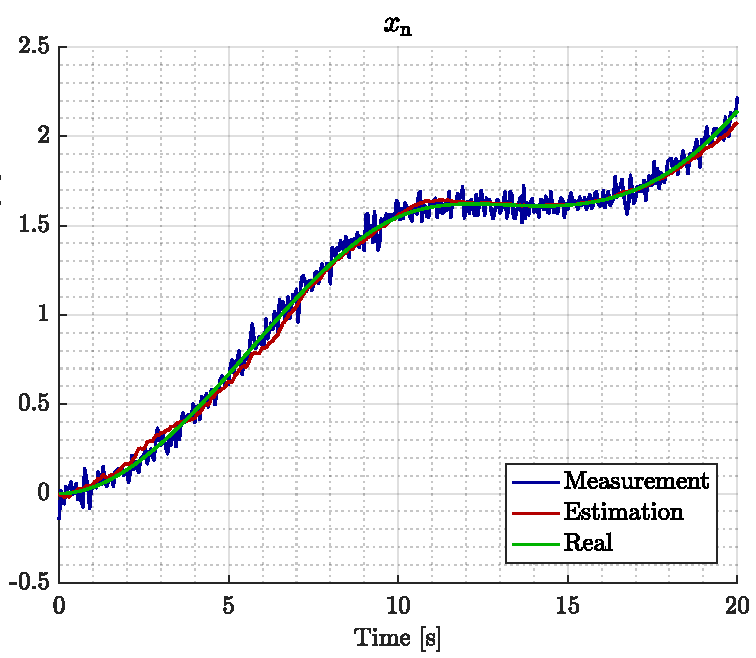
\includegraphics[width=0.5\textwidth]{figures/sim_xn}
    \caption{Measurement, real value and estimation of $x_\mathrm{n}$.}
    \label{fig:sim_xn}
\end{figure}


\begin{figure}[H]
    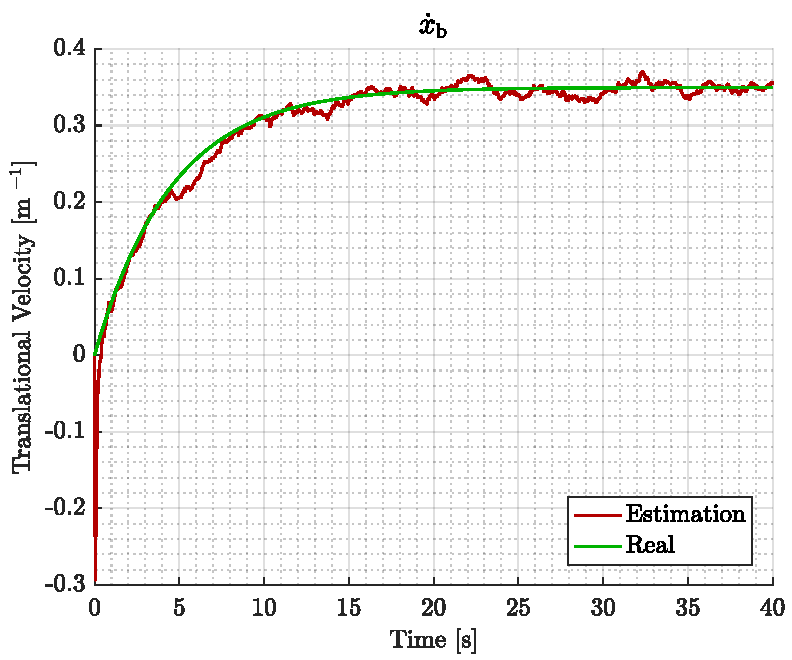
\includegraphics[width=0.5\textwidth]{figures/sim_xbdot}
    \caption{Real value and estimation of $\dot{x}_\mathrm{b}$}
    \label{fig:sim_xbdot}
\end{figure}

%\begin{figure}[H]
%    \captionbox 
%    {   
%        Result of the estimation of the translational velocity along $x_\mathrm{b}$, compared to the real value in the simulation..
%        \label{fig:sim_xbdot}
%    }                                                                 
%    {                                                                  
%        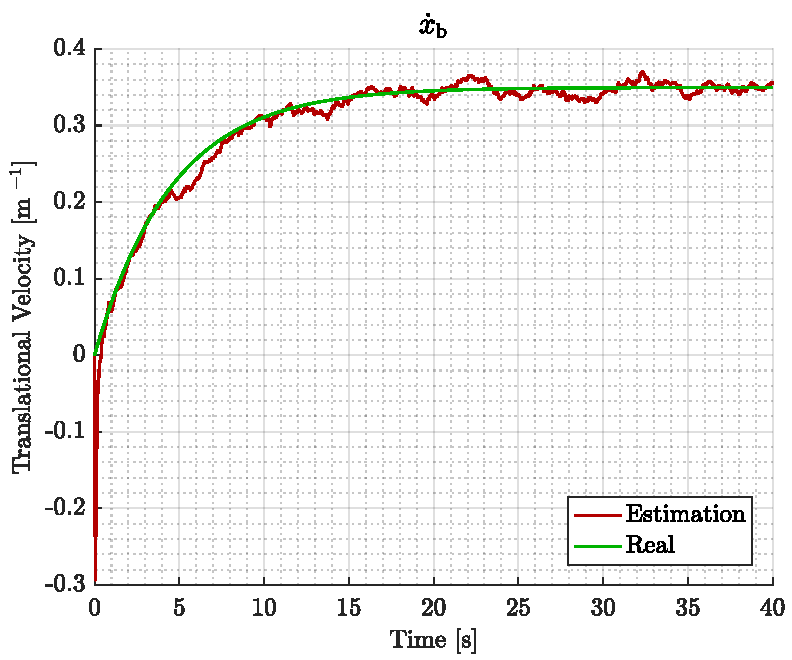
\includegraphics[width=.45\textwidth]{figures/sim_xbdot}         
%    }                                                                    
%    \hspace{5pt}                                                          
%    \captionbox  
%    {      
%        Estimation of the translational acceleration along $x_\mathrm{b}$, compared to the real value and the measurements.
%        \label{fig:sim_xbddot}
%    }                                                                          
%    {
%        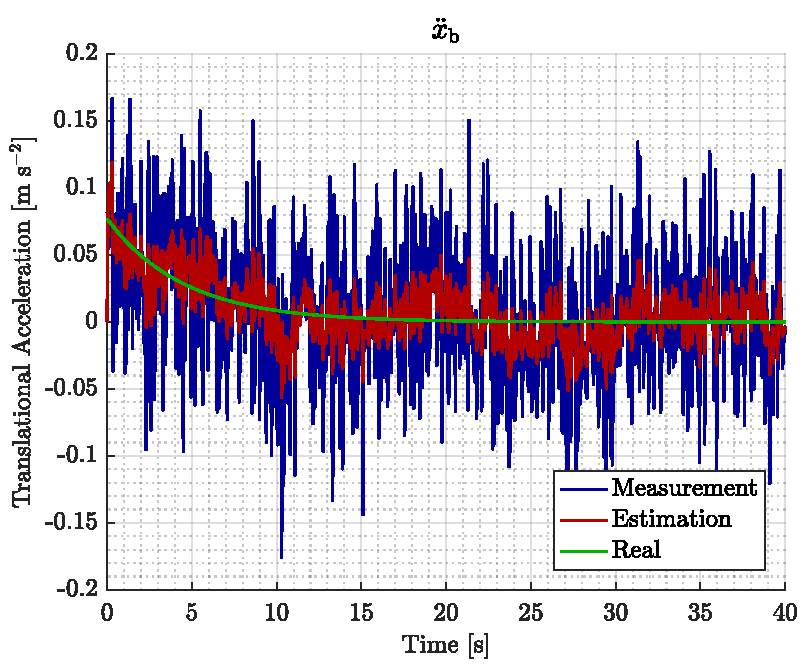
\includegraphics[width=.45\textwidth]{figures/sim_xbddot}
%    }
%\end{figure}